\chapter{Discussão de resultados}

\par Neste capítulo serão apresentados e discutidos os resultados obtidos pela pesquisa e implementação 
do sistema de otimização do processo de fabricação de calças. Tal discussão será realizada em forma de
casos de teste, buscando demonstrar o comportamento do algoritmo genético de diferentes formas.

\par Desde o princípio, quando começou-se a discutir sobre o tema do 
trabalho de conclusão de curso, teve-se a ideia de desenvolver algo relacionado
à inteligência artificial, por ser um assunto de bastante relevância na área de desenvolvimento de software. 
Dentro deste campo então, realizando algumas buscas na internet, foi encontrado
o assunto de algoritmos genéticos.
Coincidentemente foi lecionada no primeiro semestre deste ano a diciplina
sistemas especialistas, a qual o assunto foi abordado o que facilitou bastante o aprendizado.

\par Assim, como sugestão do professor orientador, foi decidido então
desenvolver uma aplicação para otimizar um processo de distribuição de atividades entre
costureiras para um microempresário da cidade de Cachoeira de Minas - MG, do ramo de costura e constatamos 
que um sistema Web seria mais cômodo de ser utilizado por não precisar de
nenhuma instalação por parte do usuário e este poder acessar o programa de
qualquer lugar desde que estivesse conectado à internet.

Neste sentido, foram adotadas como tecnologias para o desenvolvimento em
plataforma Web os \textit{frameworks} JSF e Primefaces. Além disso foi utilizado
um \textit{plug-in} denominado \texttt{JBoss Tool} o qual foi de grande utilidade para gerar as classes 
modelo a partir do banco de dados.

\par Inicialmente foi tomado como base o caso do microempresário citado acima,
todavia logo após iniciarmos o trabalho, o mesmo fez uma reestruturação de processos em sua empresa. 
Desta forma, sua maneira de trabalhar deixou de ser um cenário o qual algoritmos genéticos
pudessem ser aplicados, desta forma, fechou-se um escopo para que o trabalho
pudesse continuar, conforme descrito na seção 3.3.2 do quadro metodológico. Com
o escopo definido, o foco passou a ser na definição da estrutura dos elementos do algoritmo genético.



\par Assim, seguindo os passos descrito no quadro metodológico, foi obtido como resultado a aplicação
capaz de distribuir atividades de forma a se obter o menor custo e o menor tempo de produção, 
alcançando assim os objetivos específicos conforme mostra a Figura ~\ref{fig:tela_inicial_da_aplicação}.

\begin{figure}[h!]
	\centerline{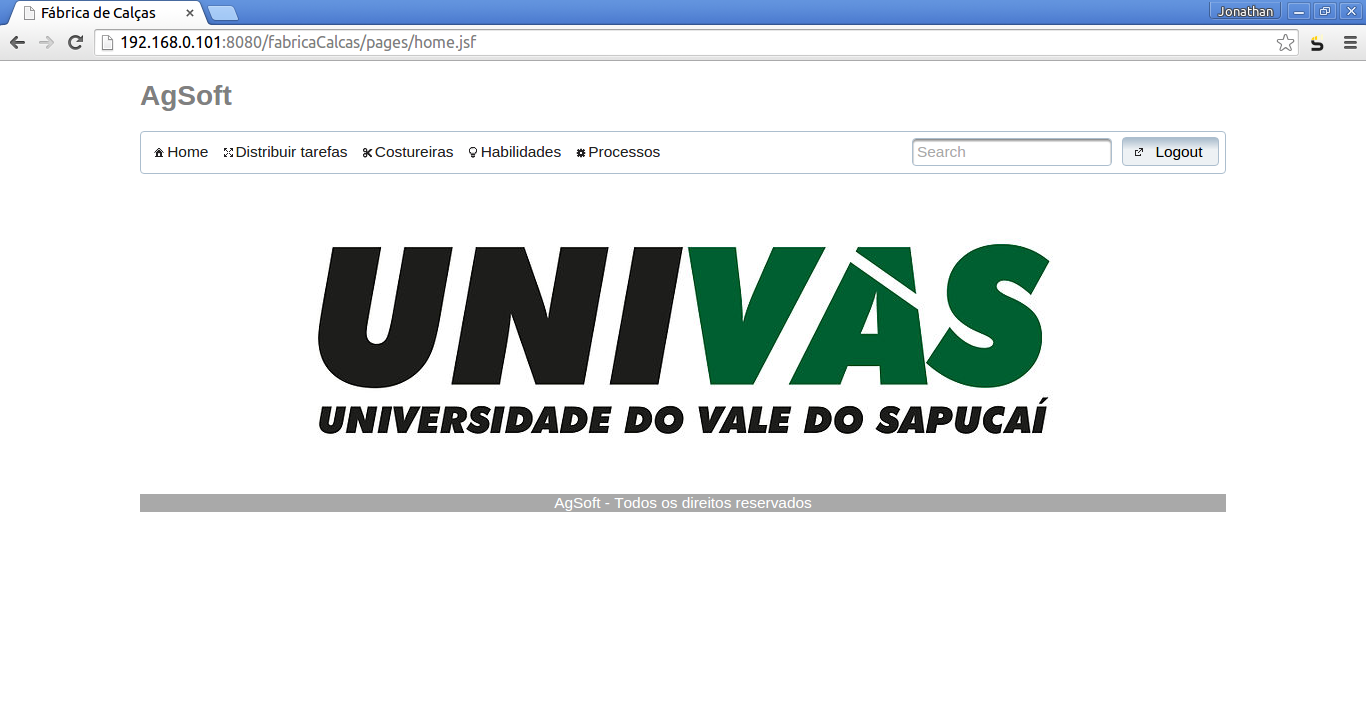
\includegraphics[scale=0.3]{./imagens/tela_inicial.png}}
	\caption[Tela inicial da aplicação]
	{Tela inicial da aplicação \textbf{Fonte:} Desenvolvido pelos autores}
	\label{fig:tela_inicial_da_aplicação}
\end{figure}


\par Com a aplicação finalizada, foram realizados então casos de testes a fim de colocar em prova a eficiência da ferramenta para se 
buscar melhores soluções nas distribuição de tarefas, conforme mostra as seções
seguintes.


\section{Teste considerando somente o tempo de produção}

\par Este teste demonstra a distribuição de lotes levando em consideração o
tempo de cada costureira para fabricação das peças. Neste teste será definido o
preço por peça igual para as costureiras alterando somente o tempo por peça de
cada uma. Para este teste foi cadastrado um processo de produção informando o
cliente, o modelo da calça e a data e hora da entrega conforme mostra a Figura 27:
\newpage

\begin{figure}[h!]
	\centerline{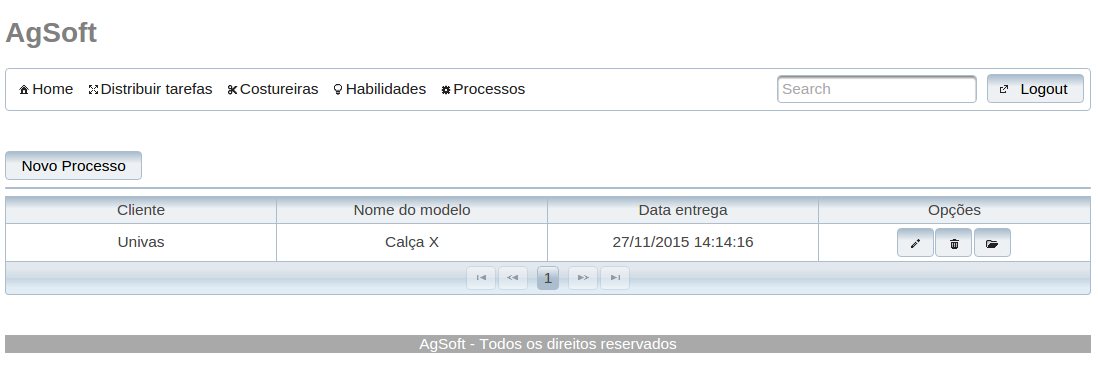
\includegraphics[scale=0.4]{./imagens/teste_processo.png}}
	\caption[Criação de um processo]
	{Criação de um processo \textbf{Fonte:} Desenvolvido pelos autores}
	\label{fig:exemplo1}
\end{figure}

\par Todo processo ao ser criado, por padrão já contém as atividades principais
 Carimbo e Finalização conforme mostra a Figura ~\ref{fig:processo_cadastrado}:

\begin{figure}[h!]
	\centerline{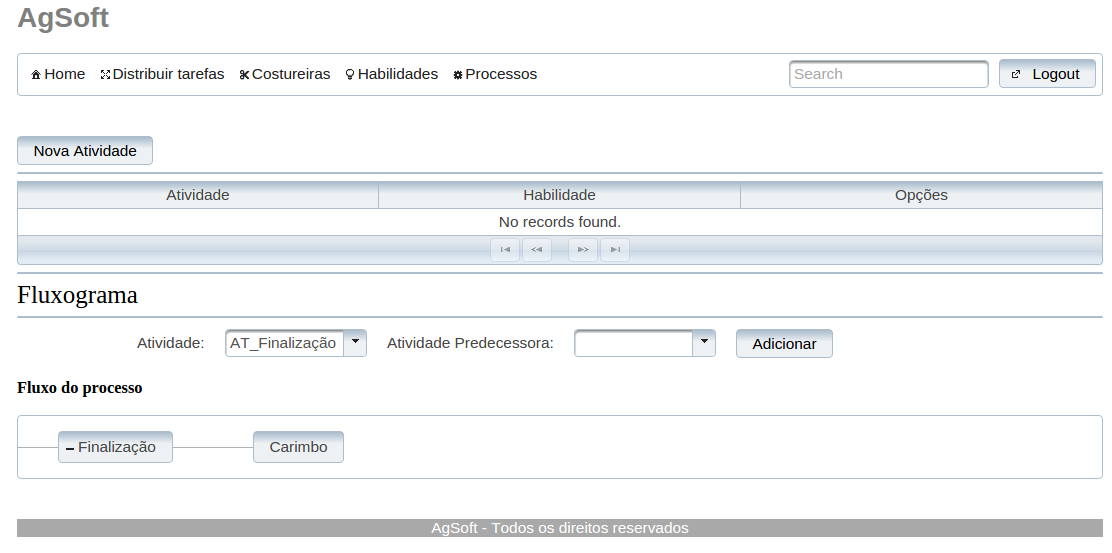
\includegraphics[scale=0.4]{./imagens/tela_processo_teste1.png}}
	\caption[Detalhes do processo cadastrado]
	{Detalhes do processo cadastrado \textbf{Fonte:} Desenvolvido pelos autores}
	\label{fig:processo_cadastrado}
\end{figure}

\par Após a criação do processo foram definidas quais costureiras possuem a
habilidade para realizar as atividades que compõe o processo, sendo definidas para 
realizar a atividade Finalização, as costureiras Maria e Duda, ambas cobram o 
mesmo valor por peça porém o tempo gasto para fabricar uma peça é diferente 
conforme mostra a Figura ~\ref{fig:costureira_habilidade}. Vale ressaltar que
a atividade Carimbo é realizada somente pelo proprietário da fábrica pois é a
atividade onde serão distribuídas as peças para serem produzidas. 

\newpage

\begin{figure}[h!]
	\centerline{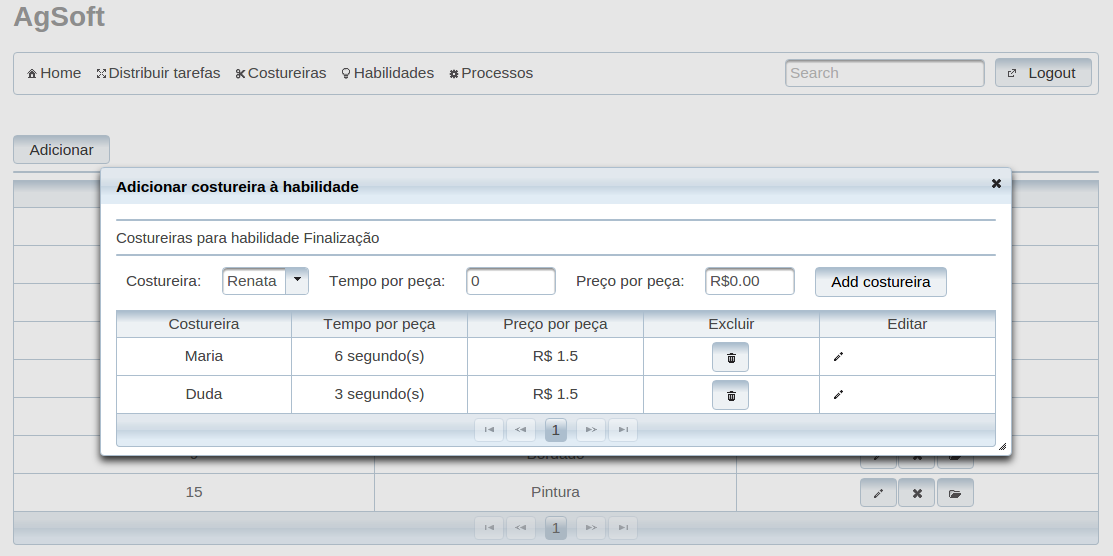
\includegraphics[scale=0.4]{./imagens/tela_habilidade_teste1.png}}
	\caption[Demonstração inserir costureira à habilidade]
	{Demonstração inserir costureira à habilidade \textbf{Fonte:} Desenvolvido pelos autores}
	\label{fig:costureira_habilidade}
\end{figure}


\par Feito isso, foi aberto o processo para a distribuição
das atividades, através do menu Distribuição de Tarefas.
Ao acessar a página todos os processos criados são
listados como mostra a Figura ~\ref{fig:distribuicao_tarefas}:

\begin{figure}[h!]
	\centerline{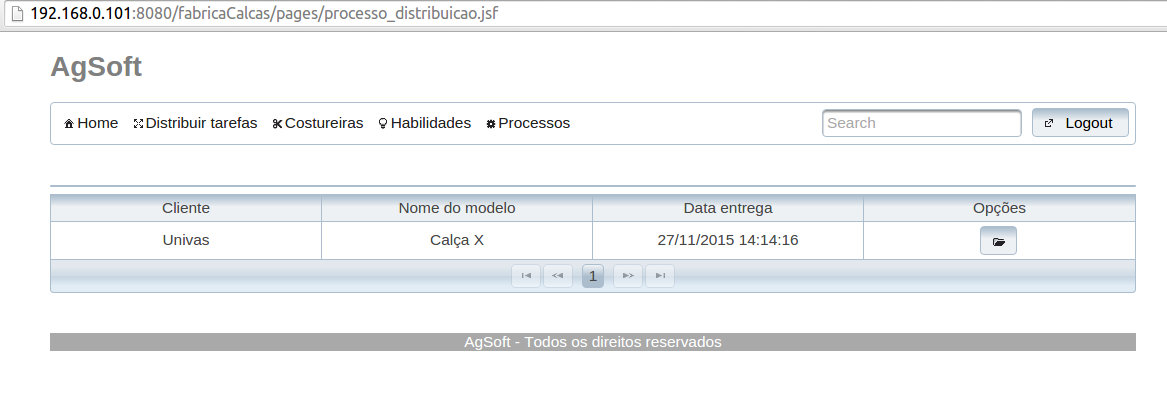
\includegraphics[scale=0.4]{./imagens/tela_distribuicao_tarefas.png}}
	\caption[Demonstração tela de dritribuição de tarefas]
	{Demonstração tela de dritribuição de tarefas \textbf{Fonte:} Desenvolvido pelos autores}
	\label{fig:distribuicao_tarefas}
\end{figure}


\par Ao clicar no botão abrir da coluna opções é mostrado a tela para que o
usuário insira os dados como número de peças, total de peças por lote e data inicio. Depois de
inseridos os dados ao clicar no botão Iniciar distribuição, o sistema executa
toda a parte de algoritmos genéticos e retorna para o usuário a melhor solução
encontrada com base nos dados inseridos conforme mostra a Figura ~\ref{fig:resultado_distribuicao_teste1}:


\begin{figure}[h!]
	\centerline{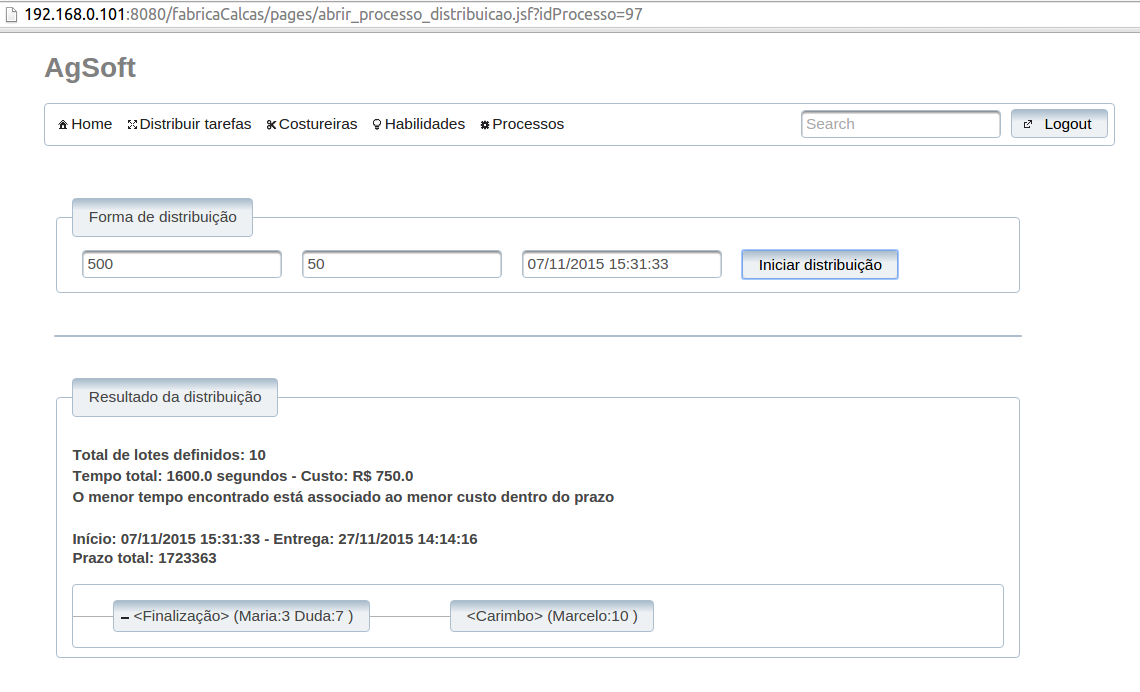
\includegraphics[scale=0.4]{./imagens/resultado_distribuicao_teste1.png}}
	\caption[Resultado da distribuição de lotes]
	{Resultado da distribuição de lotes \textbf{Fonte:} Desenvolvido pelos autores}
	\label{fig:resultado_distribuicao_teste1}
\end{figure}

\par Os valores então foram definidos, a distribuição foi realizada, e o resultado apresentado
. Conforme ilustrado na Figura ~\ref{fig:costureira_habilidade}, Maria possui
o tempo de produção maior que Duda, por isso ela recebeu um número menor de lotes
para produzir conforme ilustrado na Figura ~\ref{fig:resultado_distribuicao_teste1}

\par Se o tempo de cada costureira for alterado, um novo resultado será
retornado levando em consideração as alterações. Para isto, foi definido para
Maria o tempo de 4 segundos e para Duda o tempo de 7 segundos conforme ilustra a
Figura ~\ref{fig:tempo_costureiras}. 

\newpage

\begin{figure}[h!]
	\centerline{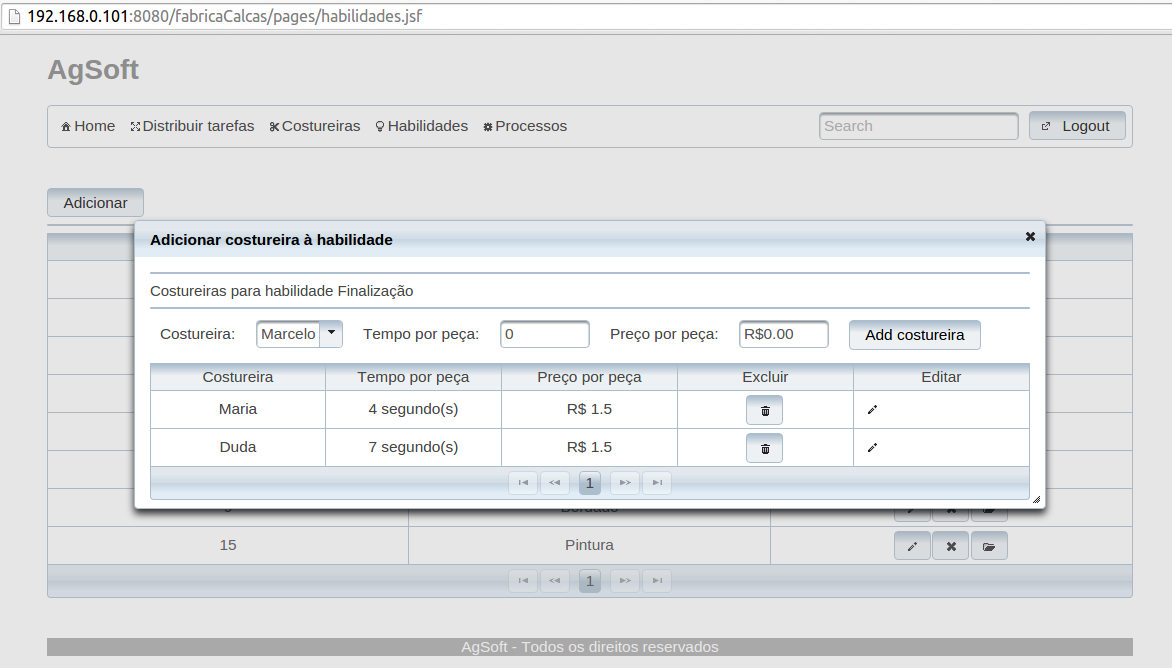
\includegraphics[scale=0.4]{./imagens/alterando_tempo_costureira.png}}
	\caption[Tempo de produção entre as costureiras]
	{Tempo de produção entre as costureiras \textbf{Fonte:} Desenvolvido pelos autores}
	\label{fig:tempo_costureiras}
\end{figure}

\par Após executar novamente a distribuição foi retornado um novo resultado
ilustrado na Figura ~\ref{fig:novo_resultado_distribuicao_teste1}:

\begin{figure}[h!]
	\centerline{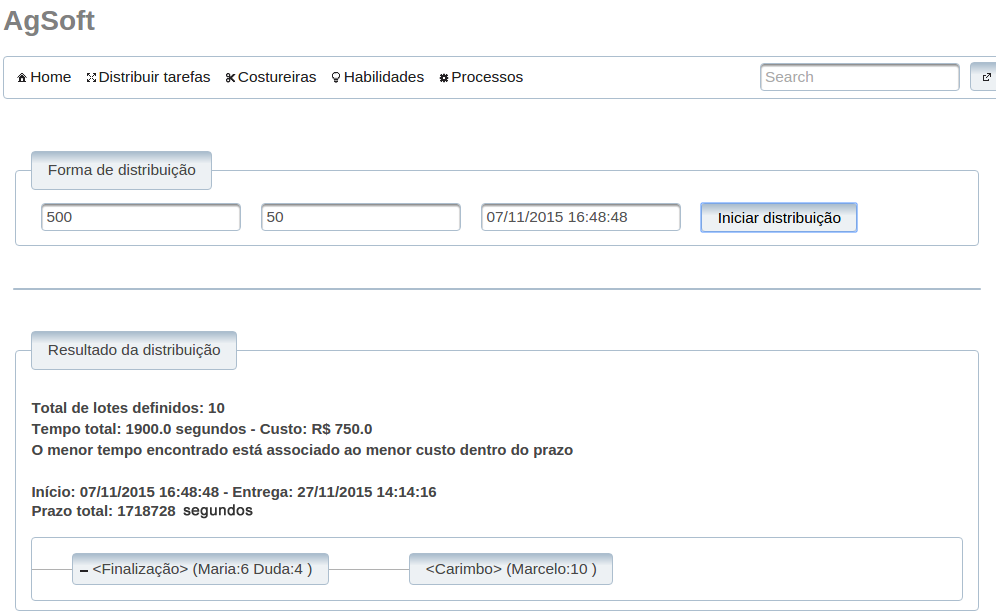
\includegraphics[scale=0.4]{./imagens/novo_resultado_alterado_tempo_teste1.png}}
	\caption[Resultado da distribuição de lotes]
	{Resultado da distribuição de lotes \textbf{Fonte:} Desenvolvido pelos autores}
	\label{fig:novo_resultado_distribuicao_teste1}
\end{figure}

\par Neste resultado Maria obteve mais lotes que Duda para produzir pois o seu tempo de produção é menor.

\section{Teste considerando o custo de produção}

\par Este teste foi realizado utilizando-se o mesmo processo do teste realizado na seção anterior,
porém foi definido o mesmo tempo de produção para ambas costureiras alterando somente o custo. Foi definido 
o tempo de 5 segundos para as costureiras Maria e Duda e o preço por peça R\textdollar 1,50 e R\textdollar 
2,70 respectivamente. Além disso foi definido os mesmos valores X e Y relativos a posição geográfica para 
Maria e Duda, de forma a manter o tempo de transporte semelhante para ambas. 
A Figura ~\ref{fig:custo_entre_costureiras} mostra a definição de tempo e custo para ambas as costureiras:



\begin{figure}[h!]
	\centerline{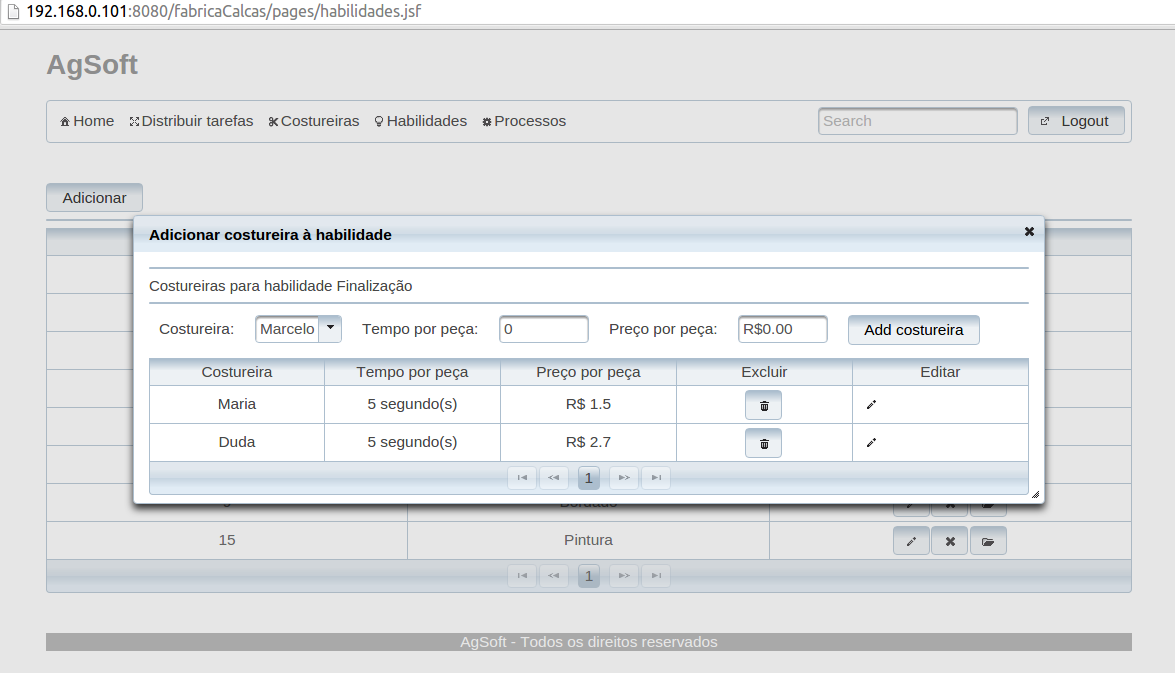
\includegraphics[scale=0.4]{./imagens/custo_entre_costureiras_teste2.png}}
	\caption[Custo entre as costureiras atividade Finalização]
	{Custo entre as costureiras atividade Finalização \textbf{Fonte:} Desenvolvido pelos autores}
	\label{fig:custo_entre_costureiras}
\end{figure}

\par Ao executar a distribuição é retornado a seguinte resultado ilustrado na Figura ~\ref{fig:resultado_custo}:

\newpage

\begin{figure}[h!]
	\centerline{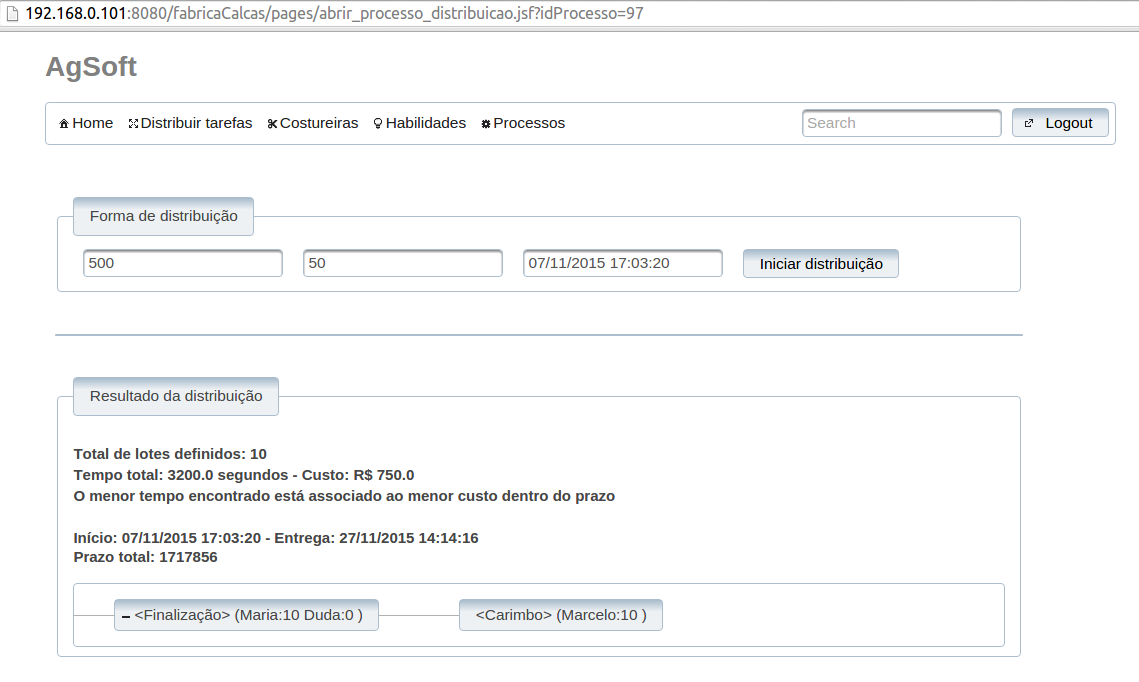
\includegraphics[scale=0.4]{./imagens/resultado_teste2.png}}
	\caption[Custo entre as costureiras atividade Finalização]
	{Custo entre as costureiras atividade Finalização \textbf{Fonte:} Desenvolvido pelos autores}
	\label{fig:resultado_custo}
\end{figure}

\par Com base no resultado obtido, o algoritmo decidiu que, pelo fato de
Maria e Duda obter o mesmo tempo de produção e Duda ter um preço por peça
bem superior que o de Maria, Duda não deve receber nenhum lote para produzir, pois neste
caso é possível que Maria produza sozinha os lotes dentro do prazo de entrega do
processo. Caso Maria não conseguisse produzir os lotes no prazo estipulado, o
algoritmo adequaria a distribuição distribuindo alguns lotes para Duda para
conseguir alcançar o prazo de entrega, toda via, fazendo isto, o custo tende a
aumentar, este caso será mostrado com mais detalhes na seção 4.3.

\par Caso Maria e Duda gastassem o mesmo tempo, cobrassem o mesmo preço e o tempo de
transporte das peças entre todos os envolvidos no processo fosse o mesmo para ambas, 
o algoritmo distribuiria lotes para Duda pois, mesmo a costureira Maria
conseguindo fabricar as peças dentro do prazo, neste caso, se Duda recebesse alguns lotes para produzir
isto não interferiria no preço final e a produção seria realizada em um tempo menor como mostra a Figura
~\ref{fig:resultado_tudo_igual}.

\newpage

\begin{figure}[h!]
	\centerline{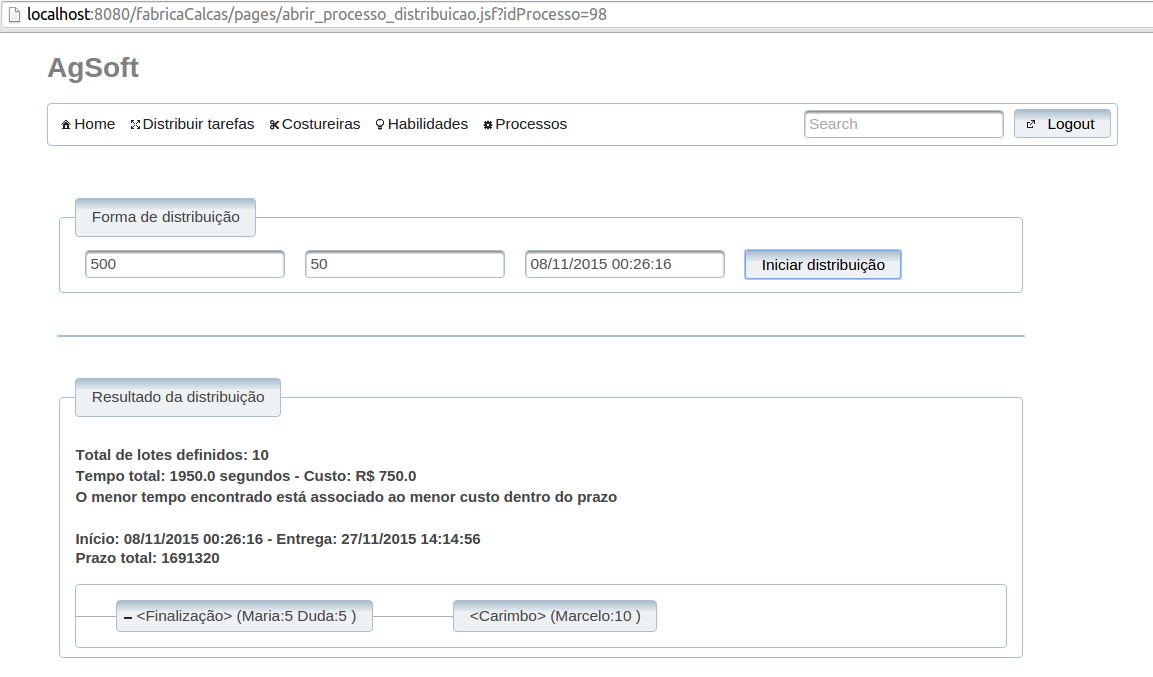
\includegraphics[scale=0.4]{./imagens/resultado_tudo_igual_teste2.png}}
	\caption[Custo entre as costureiras atividade Finalização]
	{Custo entre as costureiras atividade Finalização \textbf{Fonte:} Desenvolvido pelos autores}
	\label{fig:resultado_tudo_igual}
\end{figure}

\section{Teste considerando tempo x custo x prazo de entrega}

\par Este teste foi realizado para demonstrar a distribuição considerando o tempo de
produção, o custo e o prazo de entrega, assim mesmo que uma costureira for inviável 
quanto ao custo, ela poderá receber lotes para produzir para que seja cumprido o prazo 
de entrega. Para isto as costureiras que possuem a habilidade Finalização ficarão com
as seguintes configurações como ilustra a Figura ~\ref{fig:configuracao_habilidade_costureira_teste3}

\newpage

\begin{figure}[h!]
	\centerline{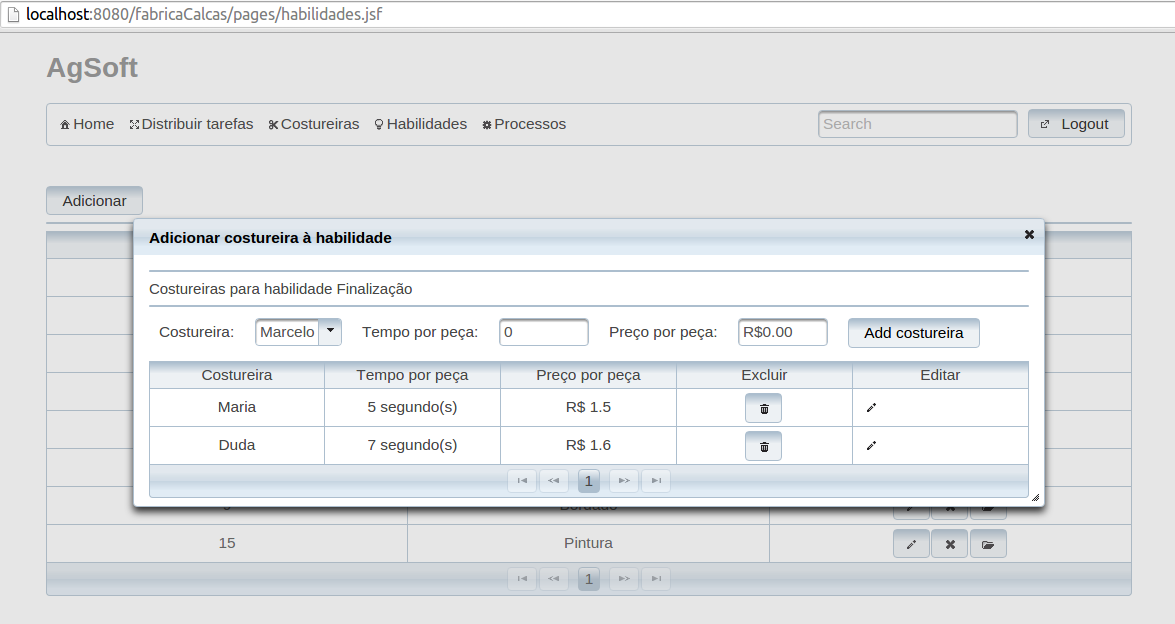
\includegraphics[scale=0.4]{./imagens/cofiguracao_habilidade_teste3.png}}
	\caption[Custo entre as costureiras atividade Finalização]
	{Custo entre as costureiras atividade Finalização \textbf{Fonte:} Desenvolvido pelos autores}
	\label{fig:configuracao_habilidade_costureira_teste3}
\end{figure}


\par A Figura ~\ref{fig:resultado1_teste3} mostra o resultado da distribuição
com base nas configurações da habilidade Finalização mostrada na Figura
~\ref{fig:configuracao_habilidade_costureira_teste3}.

\begin{figure}[h!]
	\centerline{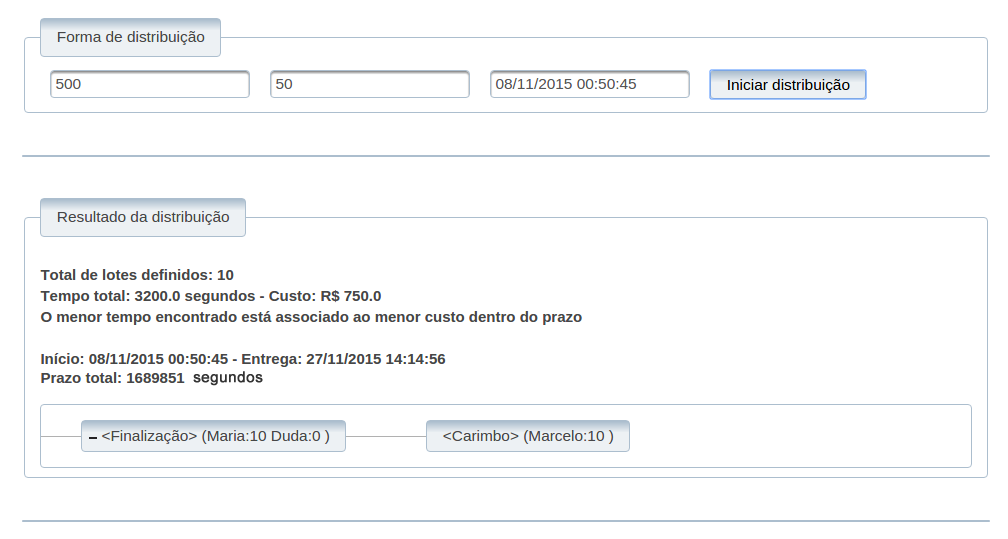
\includegraphics[scale=0.4]{./imagens/resultado1_teste3.png}}
	\caption[Custo entre as costureiras atividade Finalização]
	{Custo entre as costureiras atividade Finalização \textbf{Fonte:} Desenvolvido pelos autores}
	\label{fig:resultado1_teste3}
\end{figure}

\par Como ilustrado na Figura ~\ref{fig:resultado1_teste3}, a costureira Duda
não recebeu nenhum lote pois possui um tempo de produção e custo maior que Maria e
esta consegue cumprir o prazo de entrega, porém, caso Maria não conseguisse atender
o prazo, Duda poderia receber lotes para produzir mesmo que custo aumente.

A Figura ~\ref{fig:resultado2_teste3} mostra a distribuição de lotes entre as
costureiras com a alteração na data de inicio do processo.

\begin{figure}[h!]
	\centerline{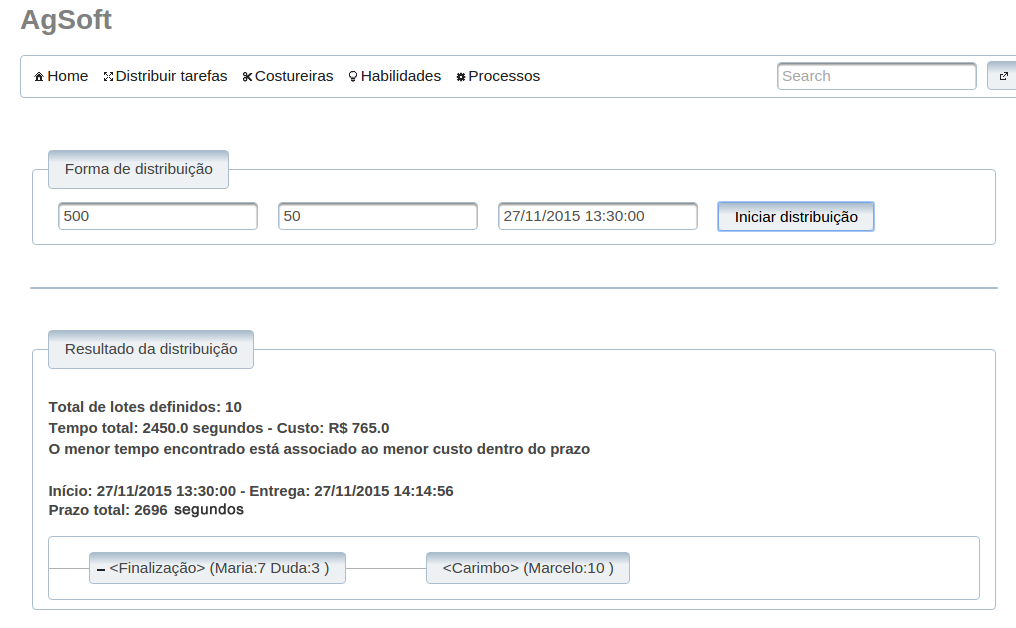
\includegraphics[scale=0.4]{./imagens/resultado2_teste3.png}}
	\caption[Custo entre as costureiras atividade Finalização]
	{Custo entre as costureiras atividade Finalização \textbf{Fonte:} Desenvolvido pelos autores}
	\label{fig:resultado2_teste3}
\end{figure}

\par Como ilustrado na Figura ~\ref{fig:resultado2_teste3} a costureira Duda
recebe 3 lotes para produzir, assim, o custo de produção aumenta com relação ao 
resultado da Figura ~\ref{fig:resultado1_teste3}, porém o tempo de produção diminui
sendo possível atender o prazo de entrega.


\section{Teste considerando o tempo de transporte}

\par Este teste foi realizado para demonstrar que mesmo as costureiras possuindo
o tempo e custo iguais, o tempo de transporte entre elas pode influenciar na distribuição dos lotes.

\par Para isto, foi necessário cadastrar um valor X e Y para cada costureira, 
conforme mostra a Figura ~\ref{fig:add_xy_costureira_teste4}.

\newpage


\begin{figure}[h!]
	\centerline{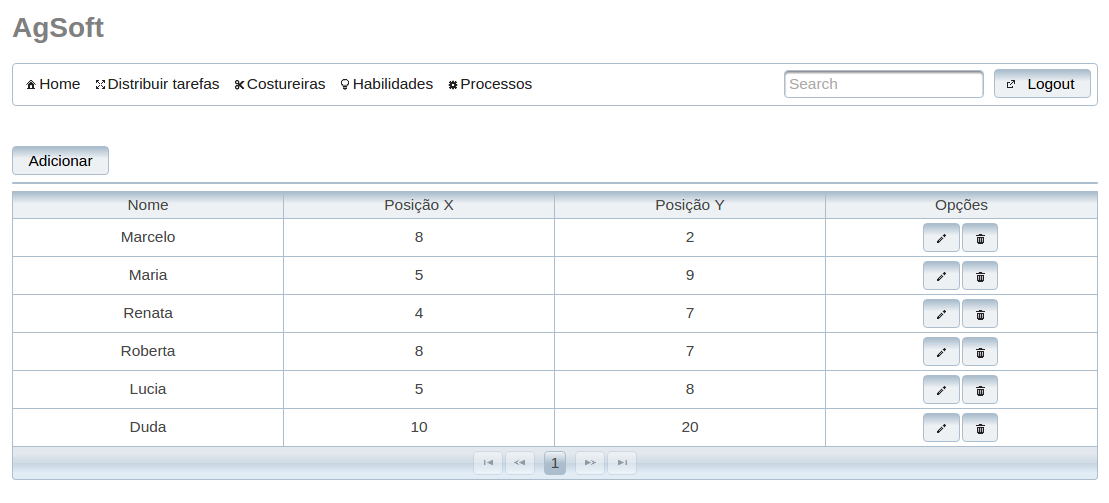
\includegraphics[scale=0.3]{./imagens/posicao_xy_costureiras_teste4.png}}
	\caption[Caso de teste com tempo de distribuição]
	{Caso de teste com tempo de distribuição \textbf{Fonte:} Desenvolvido pelos autores}
	\label{fig:add_xy_costureira_teste4}
\end{figure}



\par Neste teste foi considerado apenas o tempo de transporte, logo o tempo de
confecção por peça das costureiras da atividade Finalização possuem o mesmo
valor de tempo e custo, conforme mostra a Figura
~\ref{fig:at_finalizacao_teste4}.


\begin{figure}[h!]
	\centerline{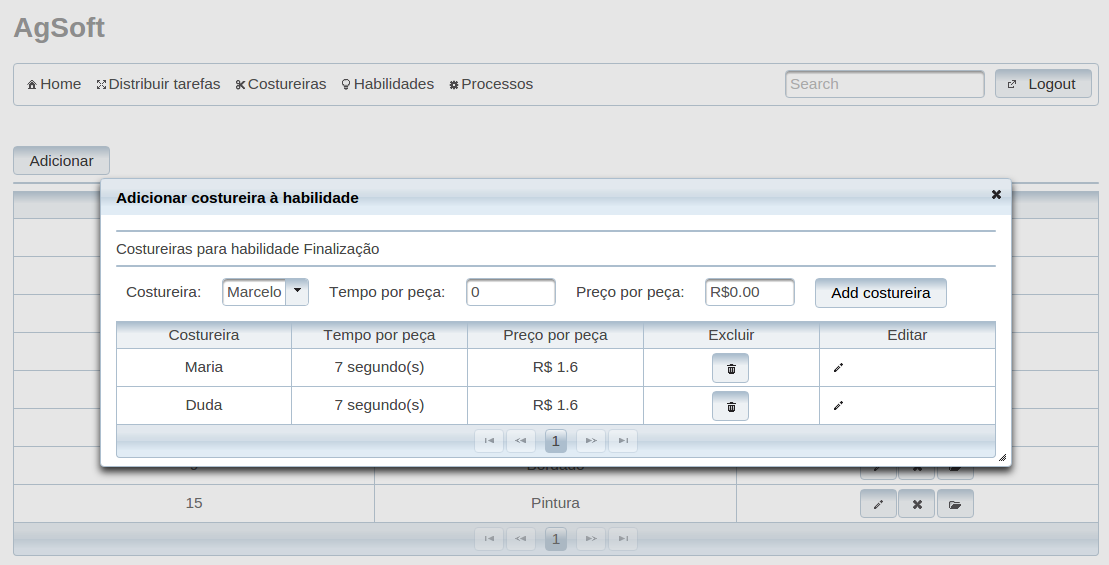
\includegraphics[scale=0.3]{./imagens/cofig_at_finalizaca_teste4.png}}
	\caption[Caso de teste com tempo de distribuição]
	{Caso de teste com tempo de distribuição \textbf{Fonte:} Desenvolvido pelos autores}
	\label{fig:at_finalizacao_teste4}
\end{figure}

\newpage

\par Feito isto, foi iniciado então o processo de distribuição das atividades,
através do menu Distribuição de Tarefas, a Figura
~\ref{fig:resultado_transporte_teste4} mostra o resultado obtido.


\begin{figure}[h!]
	\centerline{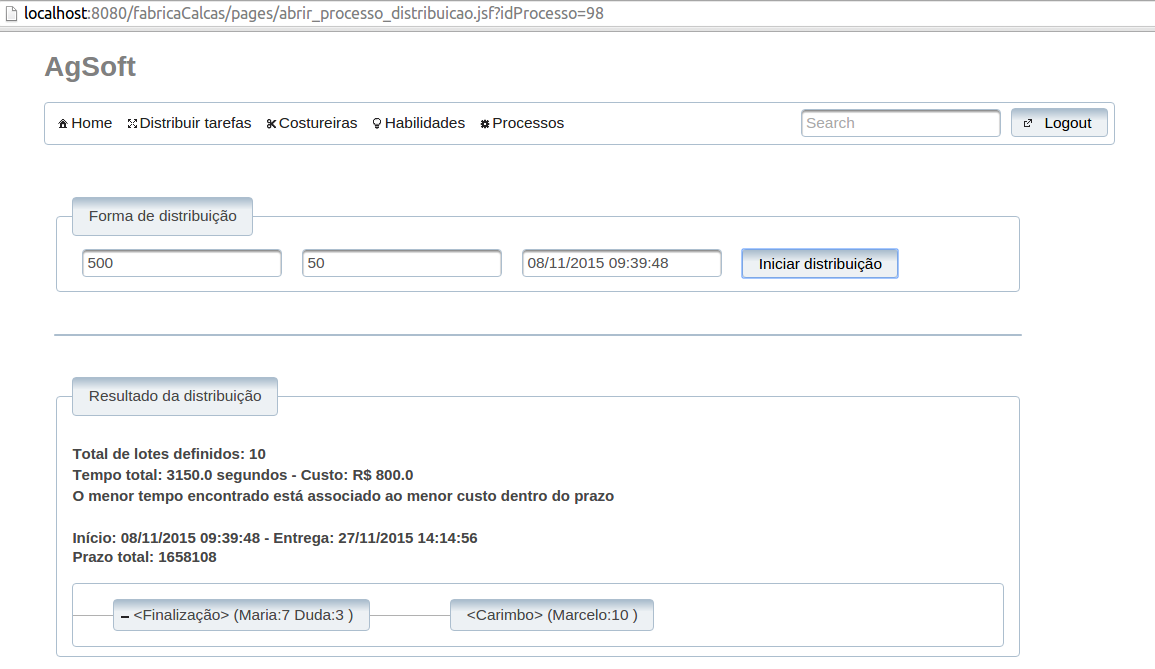
\includegraphics[scale=0.3]{./imagens/resultado_transporte_teste4.png}}
	\caption[Distribuição das atividades]
	{Distribuição das atividades \textbf{Fonte:} Desenvolvido pelos autores}
	\label{fig:resultado_transporte_teste4}
\end{figure}

\par Como mostrado na figura ~\ref{fig:add_xy_costureira_teste4}, a costureira
Duda fica mais distante do Marcelo e por isso recebe menos lotes para produzir em
relação a costureira Maria.

\par Para melhor ilustar o tempo de envio das peças para as costureiras, na tela
de resultados há um detalhamento de todo calculo realizado, a Figura
~\ref{fig:detalhameneto_transporte_teste4} mostra que o tempo de envio da peças para Duda é 
maior que o tempo de envio para Maria, comprovando o resultado mostrado na
Figura ~\ref{fig:resultado_transporte_teste4}.

\begin{figure}[h!]
	\centerline{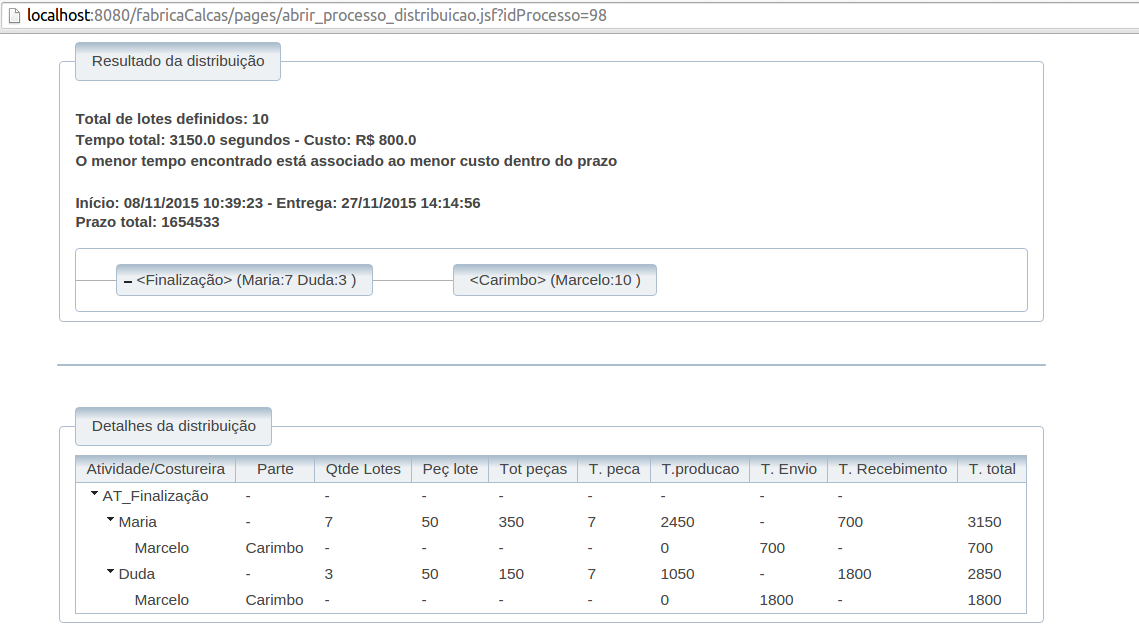
\includegraphics[scale=0.3]{./imagens/detalhamento_transporte_teste4.png}}
	\caption[Distribuição das atividades]
	{Distribuição das atividades \textbf{Fonte:} Desenvolvido pelos autores}
	\label{fig:detalhameneto_transporte_teste4}
\end{figure}

\par Como mostrado na Figura ~\ref{fig:detalhameneto_transporte_teste4}, o tempo
de envio das peças para Duda é 1800 segundos e para Maria 700, por isso
Duda recebe menos lotes para ser produzidos.


\section{Teste adicionando mais atividades ao processo}

\par Este teste foi realizado para demonstrar a adição de mais atividades no
processo. Este teste segue o mesmo processo da seção 4.1.

\par Neste caso deve-se considerar o tempo de transporte entre as costureiras da atividade Frente e o Marcelo 
para a retirada dos materiais e o tempo entre tais costureiras e a costureira
responsável pela Finalização, para isso foi adicionado no processo a atividade
Frente conforme mostra a Figura ~\ref{fig:add_frente_teste5}.

\begin{figure}[h!]
	\centerline{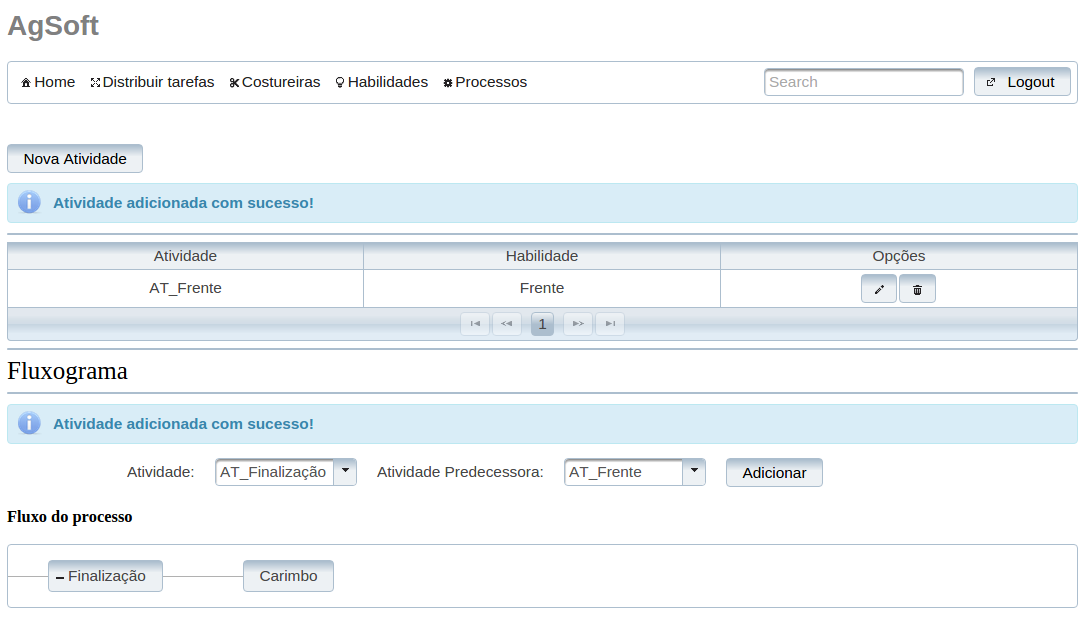
\includegraphics[scale=0.3]{./imagens/adiconar_atividade_frente_teste5.png}}
	\caption[Caso de teste com tempo de distribuição]
	{Caso de teste com tempo de distribuição \textbf{Fonte:} Desenvolvido pelos autores}
	\label{fig:add_frente_teste5}
\end{figure}

\par Após a adição da atividade, é preciso adicioná-la ao fluxo do processo como
predecessora da atividade Finalização. Como a atividade Finalização é sempre a
última atividade do processo, todas as atividades que forem incluídas sempre
serão predecessoras a ela.  A Figura ~\ref{fig:add_frente_teste4} mostra a atividade Frente adicionada
no fluxo do processo.

\newpage

\begin{figure}[h!]
	\centerline{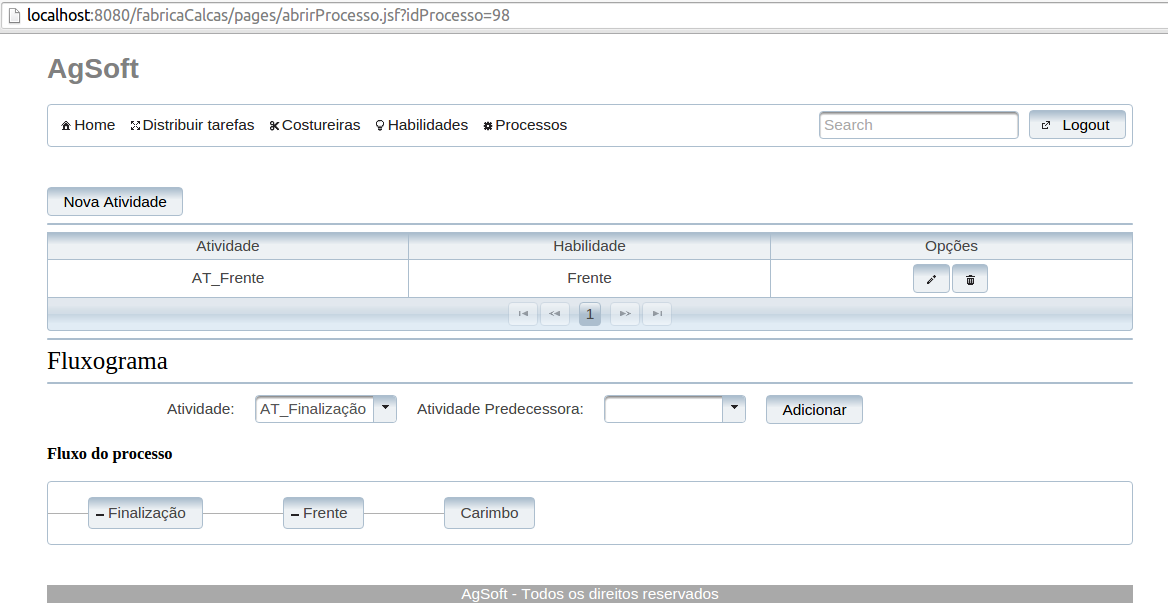
\includegraphics[scale=0.3]{./imagens/adicionar_atividade_frente_teste4.png}}
	\caption[Caso de teste com tempo de distribuição]
	{Caso de teste com tempo de distribuição \textbf{Fonte:} Desenvolvido pelos autores}
	\label{fig:add_frente_teste4}
\end{figure}


\par Foi adicionado na habilidade Frente as costureiras Roberta, Lucia e Renata
para que estas possam realizar a atividade Frente do processo.
\par A Figura ~\ref{fig:add_costureira_frente_teste4} mostra as costureiras
adicionadas na habilidade Frente.

\begin{figure}[h!]
	\centerline{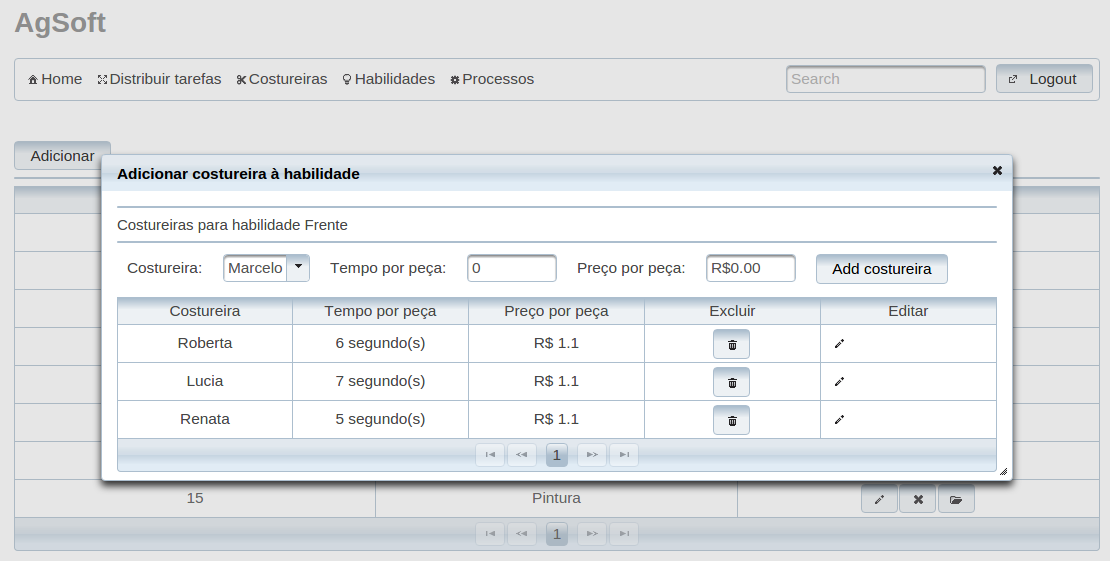
\includegraphics[scale=0.3]{./imagens/costureiras_at_frente_tete5.png}}
	\caption[Caso de teste com tempo de distribuição]
	{Caso de teste com tempo de distribuição \textbf{Fonte:} Desenvolvido pelos autores}
	\label{fig:add_costureira_frente_teste4}
\end{figure}

\par Feito isso foi realizado a distribuição dos lotes com as configurações de
tempo e custo mostradas na Figura ~\ref{fig:add_costureira_frente_teste4} e com
as configurações de posicionamento mostradas na Figura
~\ref{fig:add_xy_costureira_teste4}.
\par A Figura ~\ref{fig:resultado1_teste5} mostra o resultado obtido na
distribuição.

\newpage

\begin{figure}[h!]
	\centerline{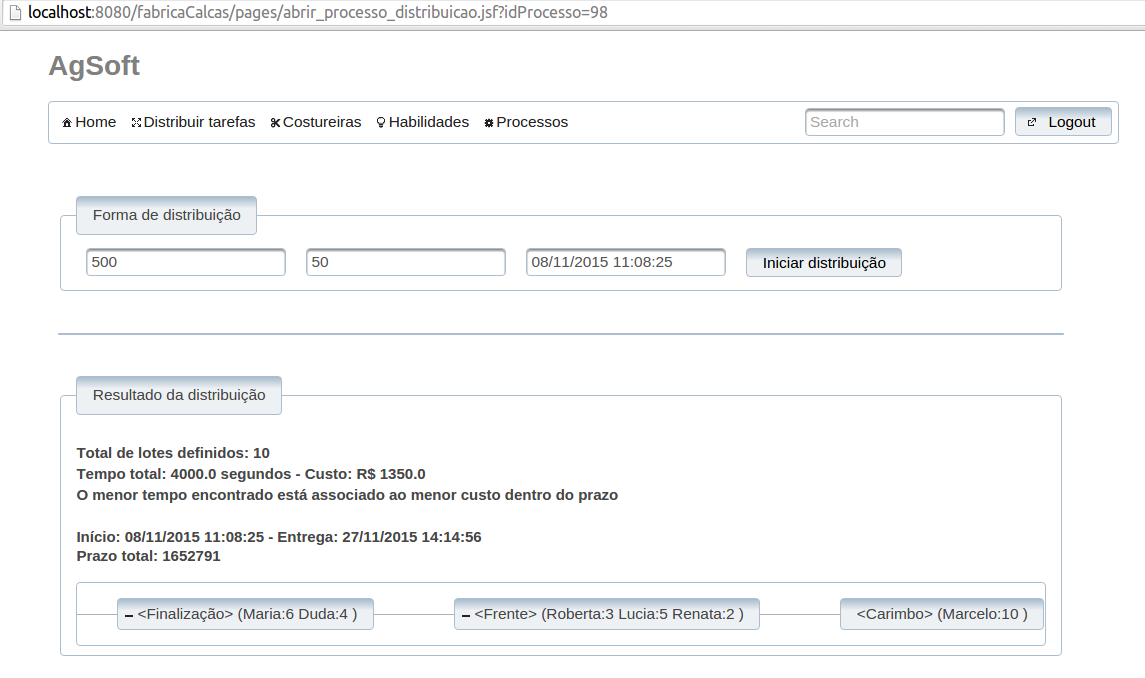
\includegraphics[scale=0.3]{./imagens/resultado1_teste5.png}}
	\caption[Caso de teste com tempo de distribuição]
	{Caso de teste com tempo de distribuição \textbf{Fonte:} Desenvolvido pelos autores}
	\label{fig:resultado1_teste5}
\end{figure}

\par Com base na Figura ~\ref{fig:resultado1_teste5} pode-se observar que foi
adicionado no resultado final a atividade Frente e suas respectivas costureiras.

\par A Figura ~\ref{fig:detalhamento1_teste5} mostra o detalhamento da
distribuição da Figura ~\ref{fig:resultado1_teste5}.

\begin{figure}[h!]
	\centerline{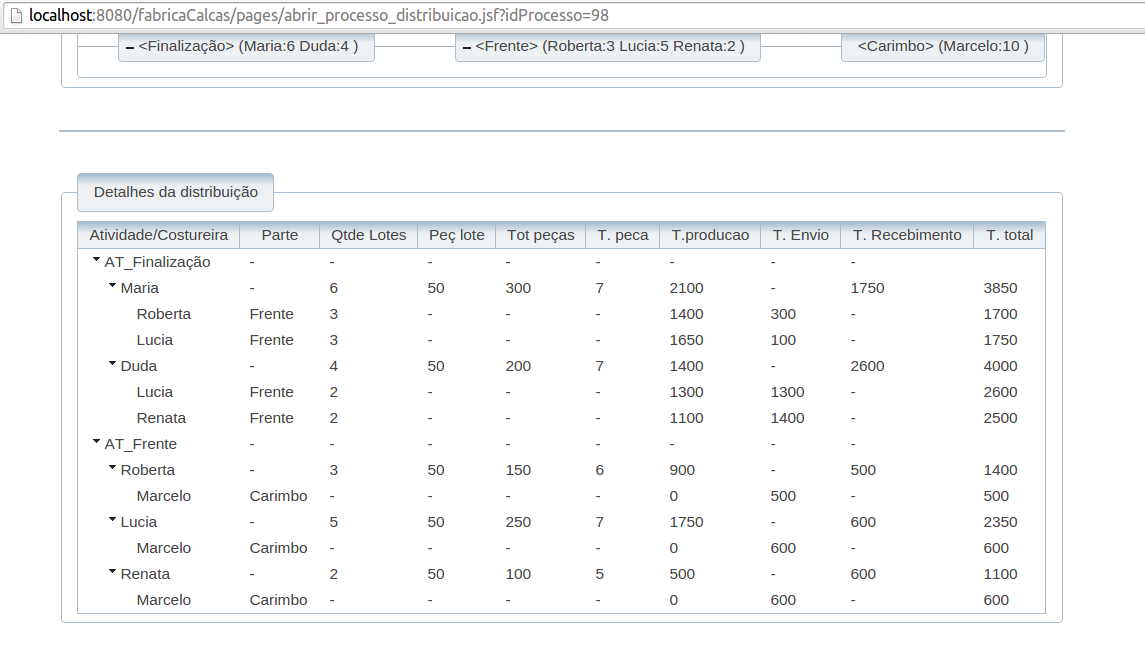
\includegraphics[scale=0.3]{./imagens/detalhamento1_teste5.png}}
	\caption[Caso de teste com tempo de distribuição]
	{Caso de teste com tempo de distribuição \textbf{Fonte:} Desenvolvido pelos autores}
	\label{fig:detalhamento1_teste5}
\end{figure}

\par Vale ressaltar que ao executar a distribuição o algoritmo pode
encontrar várias soluções que contém o mesmo resultado e retorna uma delas, se a
distribuição for executada novamente mantendo as configurações das costureiras
como a posição X e Y, tempo e custo, a distribuição poderá ocorrer de uma outra
forma conforme mostra a Figura ~\ref{fig:resultado2_teste5}.

\newpage

\begin{figure}[h!]
	\centerline{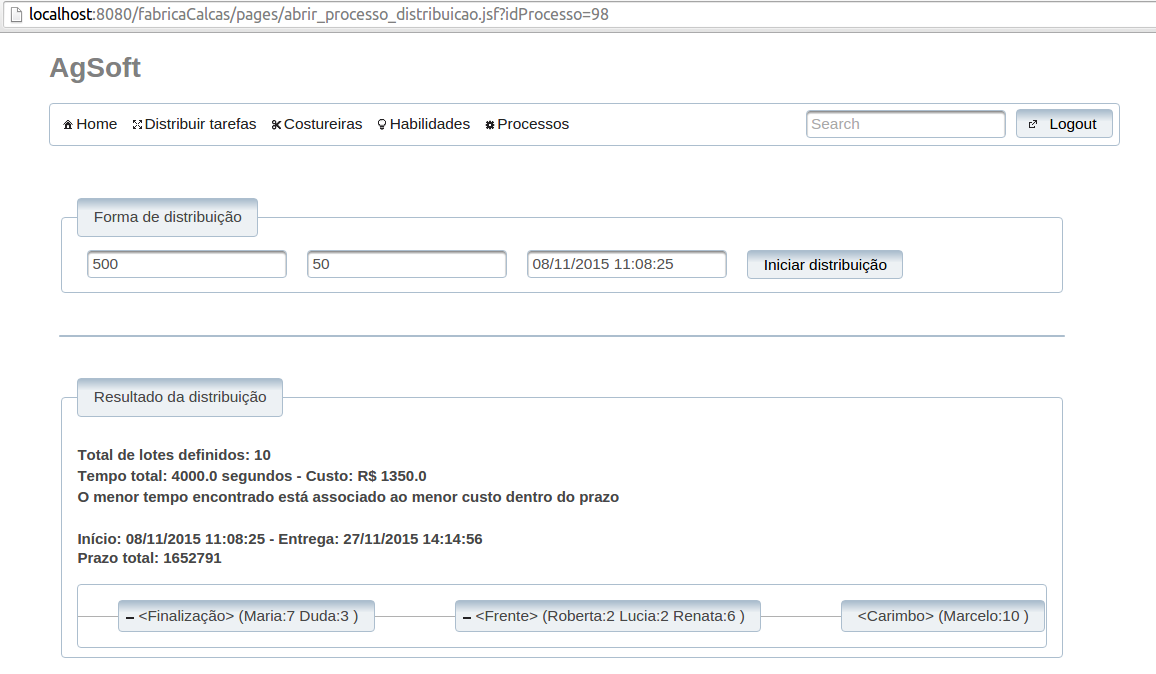
\includegraphics[scale=0.3]{./imagens/resultado2_teste5.png}}
	\caption[Caso de teste com tempo de distribuição]
	{Caso de teste com tempo de distribuição \textbf{Fonte:} Desenvolvido pelos autores}
	\label{fig:resultado2_teste5}
\end{figure}


\par A Figura ~\ref{fig:detalhamento2_teste5} mostra o detalhamento da
distribuição da Figura ~\ref{fig:resultado2_teste5}.



\begin{figure}[h!]
	\centerline{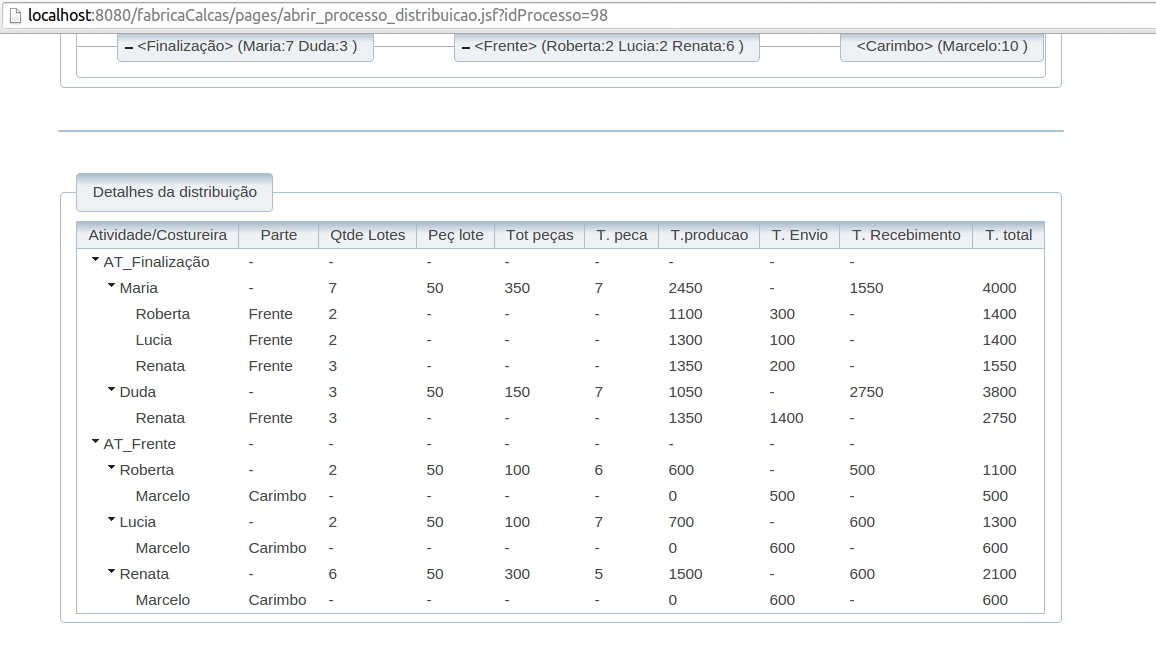
\includegraphics[scale=0.3]{./imagens/detalhamento2_teste5.png}}
	\caption[Caso de teste com tempo de distribuição]
	{Caso de teste com tempo de distribuição \textbf{Fonte:} Desenvolvido pelos autores}
	\label{fig:detalhamento2_teste5}
\end{figure}


\par Com base nas Figuras ~\ref{fig:resultado1_teste5} e
~\ref{fig:resultado2_teste5} pode-se observar que o tempo total de produção e o
custo final não tiveram alterações de uma distribuição para outra, porém a
distribuição dos lotes entre as costureiras é realizado de uma forma
diferente, concluindo assim que o algoritmo encontrou outra forma de realizar a
distribuição mantendo o melhor resultado.
